\chapter{函数插值和重构}
\label{chap:interpolation}

\paragraph{基本问题}
已知关于某函数$f$的一组信息,如何重构$f$?事实上,由于信息缺失,无法准确重构。

\begin{definition}
    {重构}{}
    给定函数空间$X$上的一组线性无关泛函$\phi_1,\ldots,\phi_n$,$f\in X$且$\phi_i(f)$已知,希望确定$f^*\in Y\subset X$满足:
    \begin{equation}
        \phi_i(f^*)=\phi_i(f),\quad i=1,\ldots,n.
    \end{equation}
    $Y$称为插值空间或重构空间,$\{\phi_i\}$为信息泛函。
\end{definition}

% \begin{remark}
%     几个基本问题:
%     \begin{itemize}
%         \item 存在性和唯一性;
%         \item 算法;
%         \item 合理性。
%     \end{itemize}
% \end{remark}

\begin{example}
    {采样空间的选择}{}
    \begin{itemize}
        \item 多项式函数空间
        \[
            \poly_n=\{a_0+a_1x+\cdots+a_nx^n\},
        \]
        \item 样条函数(spline)空间:分段多项式函数;
        \item 三角多项式函数空间
        \[
            \mathcal Y_n=\{a_0+a_1\cos x+b_1\sin x+\cdots+a_n\cos nx+b_n\sin nx\}.
        \]
    \end{itemize}
\end{example}

\section{一维多项式插值}
\label{sec:1-D polynomial interpolation}

\subsection{Lagrange插值}

\begin{definition}
    {Lagrange插值}{Lagrange interpolation}
    插值空间$Y$由$n+1$个参数$a_0,\ldots,a_n$标定,即
    \[
        y=y(x;a_0,\ldots,a_n).
    \]
    给定一组插值节点(采样点) $x_i$和采样值$f_i=f(x_i)$,希望确定参数满足
    \begin{equation}
        y(x_i)=f(x_i),\quad\forall i\in I.
    \end{equation}
\end{definition}

\begin{theorem}
    {多项式插值定理}{}
    给定$n+1$个不同插值点$x_0,\ldots,x_n$,存在唯一的多项式函数$p_n\in\poly_n$满足插值条件。
\end{theorem}
\begin{proof}
    存在性:
    采取直接构造的方法。
    定义插值基函数$\ell_i\in\poly_n$:
    \begin{equation}
        \label{eqn:Lagrange base}
        \ell_i(x):=\prod_{j\neq i}\frac{x-x_j}{x_i-x_j}.
    \end{equation}
    易验证,$\ell_i$满足:
    \begin{equation}
        \ell_i(x_j)=\delta_{ij}.
    \end{equation}
    故插值多项式为
    \begin{equation}
        \label{eqn:Lagrange polynomial}
        p_n(x)=\sum_{i=0}^nf(x_i)\ell_i(x).
    \end{equation}
    唯一性:
    若还存在$q_n\in\poly_n$满足插值条件,则$p_n-q_n\in\poly_n$且有$x_0,\ldots,x_n$共$n+1$个零点,故$p_n-q_n\equiv 0$。
\end{proof}

\begin{definition}
    {余项}{remainder}
    定义插值函数$p_n(x)$与被插值函数$f(x)$之间的差为余项(remainder)
    \begin{equation}
        R_n(x):=f(x)-p_n(x).
    \end{equation}
\end{definition}

\begin{theorem}
    {中值定理与余项}{mean value theorem of remainder}
    若$f\in\cont^{n+1}[a,b]$,则$\forall x\in[a,b],\exists\xi(x)\in(a,b)$使得
    \begin{equation}
        \label{eqn:Lagrange remainder}
        R_n(x)=\frac{f^{(n+1)}(\xi(x))}{(n+1)!}\prod_{i=0}^n(x-x_i).
    \end{equation}
\end{theorem}

\begin{proof}
    当$x=x_i$时,$R_n(x_i)=0$显然成立;
    给定$x\in[a,b]$且$x\neq x_i$,定义
    \[
        g(t):=R_n(t)-\frac{\prod_{i=0}^n(t-x_i)}{\prod_{i=0}^n(x-x_i)}R_n(x),
    \]
    则$g\in\cont^{n+1}[a,b]$且在$[a,b]$上有$x_0,\ldots,x_n,x$共$n+2$个零点,在其划分的$n+1$个区间中应用Rolle定理:对应存在$\xi_1^{(1)},\ldots,\xi_{n+1}^{(1)}$使得
    \[
        g'(\xi_i^{(1)})=0,\quad i=0,1,\ldots,n+1,
    \]
    继续对$\xi_0^{(1)},\ldots,\xi_{n+1}^{(1)}$划分的$n$个区间上应用Rolle定理,直到$g^{(n+1)}(\xi^{(n+1)}_0)=0$:
    \[
        g^{(n+1)}(\xi^{(n+1)}_0)=f^{(n+1)}(\xi^{(n+1)}_0)-\frac{(n+1)!}{\prod_{i=0}^n(x-x_i)}R_n(x)=0.
    \]
    取$\xi=\xi_0^{(n+1)}$即证。
\end{proof}

\begin{corollary}
    若$f\in\cont^{n+1}[a,b]$,$h=\max(x_{i+1}-x_i)$则
    \begin{equation}
        \norm{R_n}_\infty\leq\frac{h^{n+1}}{4(n+1)}\norm{f^{(n+1)}}_\infty.
    \end{equation}
\end{corollary}

\subsection{Lagrange插值的收敛性}

当什么条件下,$n\to\infty$,误差$\norm{R_n}_\infty\to 0$?

\begin{theorem}
    {Lagrange插值收敛性的一个充分条件}{}
    若被插值函数的任意阶导数一致有界,则误差收敛到0。
\end{theorem}

\begin{example}
    {}{}
    给定$f(x)=\sin x,\enspace x\in[0,\pi]$,由于$\forall x\in[0,\pi]$
    \[
        \abs{f^{(n+1)}(x)}\leq 1,\quad\abs{\prod_{i=0}^n(x-x_i)}\leq\pi^{n+1},
    \]
    故
    \[
        \abs{R_n(x)}\leq\frac{\pi^{n+1}}{(n+1)!}\to0,
    \]
    说明Lagrange插值多项式$p_n$在$[0,\pi]$上一致收敛到$f$。
\end{example}

% \begin{theorem}
%     {误差收敛性的一个充分条件}{}
%     记$\delta:=\abs{I(x_0,\ldots,x_n)}$,$\tilde x$为$I$的中心。如果$f$在$B(\tilde x,2\delta)$上复解析,则插值法在$I$上是收敛的。
% \end{theorem}

% \begin{proof}
%     设$M$为$f$在$\Omega=B(\tilde x,1.9\delta)$上的上界,则
%     \begin{equation}
%         \frac{f^{n+1}(\xi)}{(n+1)!}=\frac1{2\pi\i}\oint_{\p\Omega}\frac{f(z)}{(z-\xi)^{n+2}}\d z,
%     \end{equation}
%     于是
%     \begin{equation*}
%         \abs{R_n(x)}\leq C\delta\frac{\delta^{n+1}}{(1.4\delta)^{n+2}}\to 0.
%         \qedhere
%     \end{equation*}
% \end{proof}

\begin{example}
    {Runge现象}{Runge's phenomenon}
    Runge函数$f(x)=\frac1{1+25x^2}$在$[-1,1]$上等距插值。
    \begin{center}
        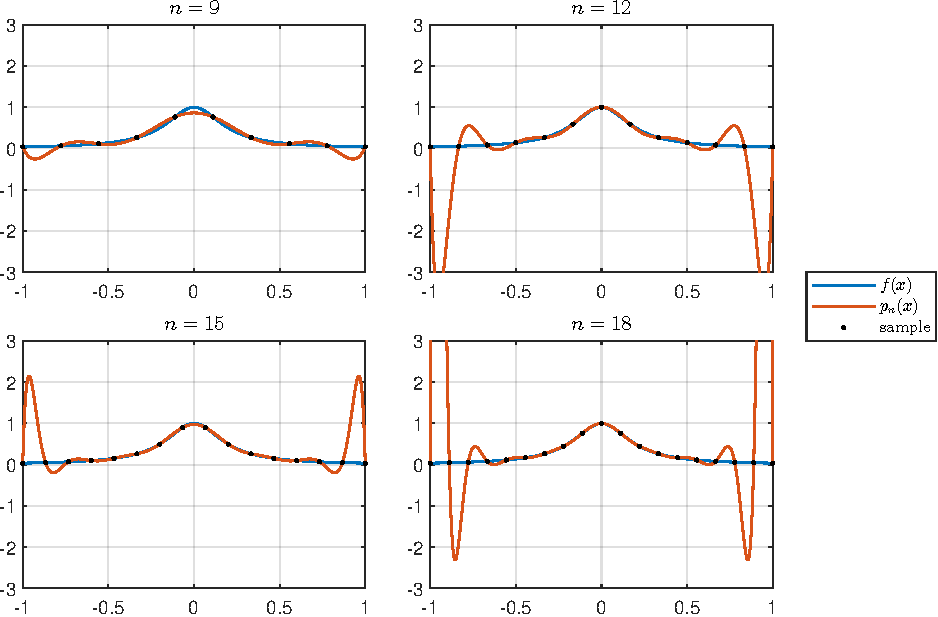
\includegraphics[width=0.9\linewidth]{graphs/Runge.pdf}
        \captionof{figure}{等距插值Runge现象}
    \end{center}
    显然$f(x)$在$\RR$上是解析的,但在$\CC$上存在奇点$\pm\i/5$。
    \tcblower
    改用$n+1$阶Chebyshev多项式零点
    \[
        \cos\biggkh{\frac{\pi}{2(n+1)}},\enspace
        \cos\biggkh{\frac{3\pi}{2(n+1)}},\enspace
        \ldots,\enspace
        \cos\biggkh{\frac{2n+1}{2(n+1)}\pi},
    \]
    作为插值节点,可以消去Runge现象。
    \begin{center}
        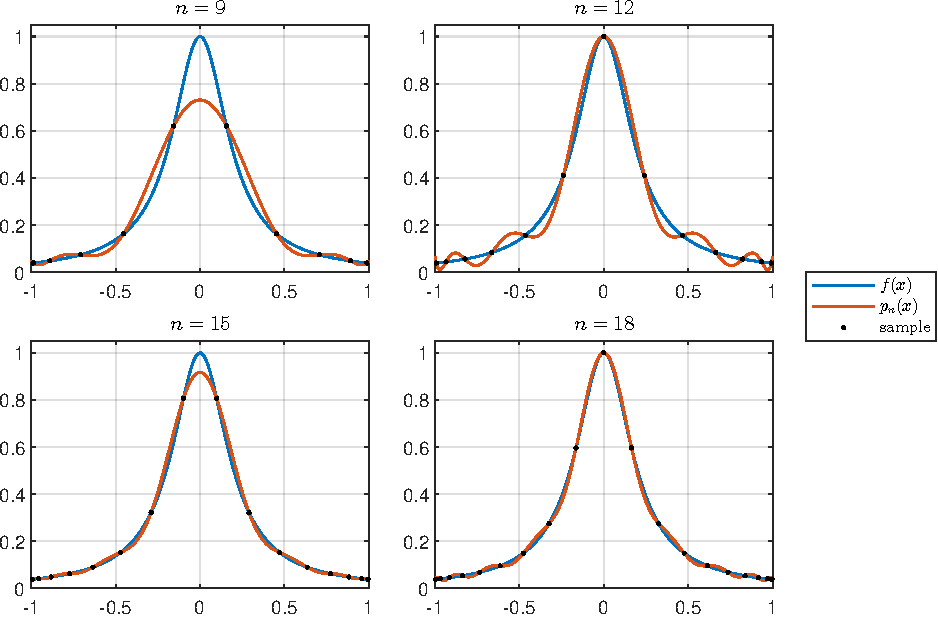
\includegraphics[width=0.9\linewidth]{graphs/Rungeless.pdf}
        \captionof{figure}{Chebyshev多项式零点插值}
    \end{center}
\end{example}

\subsection{Newton插值公式}

\iffalse
\begin{table}[h]
    \centering
    \begin{tabular}{cccc}
        \toprule
        0&1&2&3\\
        \midrule 
        \begin{tabular}[c]{@{}c@{}}
            $P_0$\\$P_1$\\$P_2$\\$P_3$
        \end{tabular} & 
        \begin{tabular}[c]{@{}c@{}}
            $P_{01}$\\$P_{12}$\\$P_{23}$
        \end{tabular} & 
        \begin{tabular}[c]{@{}c@{}}
            $P_{012}$\\$P_{123}$
        \end{tabular} & $P_{0123}$ \\
        \bottomrule
    \end{tabular}
\end{table}
\fi

\begin{definition}
    {均差}{divided differences}
    定义$f$在节点集$i_0,i_1,\ldots,i_k$上的$k$阶均差(divided differences)递归地定义为:
    \begin{equation}
        f[x_{i_0},\ldots,x_{i_k}]:=\frac{f[x_{i_1},\ldots,x_{i_k}]-f[x_{i_0},\ldots,x_{i_{k-1}}]}{x_{i_k}-x_{i_0}}.
    \end{equation}
    特别地,$f$在$x_i$上的零阶均差$f[x_i]:=f(x_i)$。
\end{definition}

\begin{corollary}
    $k$阶均差$f[x_0,\ldots,x_k]$是$f(x_0),\ldots,f(x_k)$的线性组合:
    \begin{equation}
        f[x_0,\ldots,x_k]=\sum_{i=0}^k\frac{f(x_i)}{\prod_{j\neq i}(x_i-x_j)}.
    \end{equation}
    因此,均差对于节点是对称的,即任意改变节点的顺序,均差的值不变。
\end{corollary}

% 如果$f$足够光滑,则
% \begin{equation}
%     \lim_{\epsilon_i\to0}f[x_0^{\epsilon_0},\ldots,x_n^{\epsilon_n}]=f[x_0,\ldots,x_n],
% \end{equation}

\begin{theorem}
    {Newton插值公式}{}
    利用均差迭代得到$n$次Newton插值多项式:
    \begin{equation}
        p_n(x)=f(x_0)+f[x_0,x_1](x-x_0)+\cdots+f[x_0,\ldots,x_n](x-x_0)\cdots(x-x_{n-1}).
    \end{equation}
    其余项为
    \begin{equation}
        R_n(x)=f[x,x_0,\ldots,x_n](x-x_0)\cdots(x-x_n).
    \end{equation}
    % \begin{equation}
    %     \begin{aligned}
    %         P_{i_0\cdots i_k}(x)&=P_{i_0\cdots i_{k-1}}(x)+f[x_{i_0},\ldots,x_{i_k}](x-x_{i_0})\cdots(x-x_{i_{k-1}})\\
    %         &=f[x_{i_0}]+f[x_{i_0},x_{i_1}](x-x_{i_0})+\cdots\\
    %         &\qqquad~+f[x_{i_0},\ldots,x_{i_k}](x-x_{i_0})\cdots(x-x_{i_{k-1}}).
    %     \end{aligned}
    % \end{equation}
\end{theorem}

对均差形式的余项应用\thmref{thm:mean value theorem of remainder} 得到:

\begin{theorem}
    {中值定理与均差}{mean value theorem of divided differences}
    如果$f\in\cont[a,b],\enspace x_0,\ldots,x_n\in[a,b]$,则$\exists\xi\in I(x_0,\ldots,x_n)$,
    \begin{equation}
        f[x_0,\ldots,x_n]=\frac{f^{(n)}(\xi)}{n!}.
    \end{equation}
\end{theorem}

\begin{corollary}
    特别地,$n$阶均差:
    \begin{equation}
        f[\underbrace{x,\ldots,x}_{n+1}]=\frac{f^{(n)}(x)}{n!}
    \end{equation}
\end{corollary}
\begin{corollary}
    均差的导数:
    \begin{equation}
        \dd xf[x_0,\ldots,x_n,x]=f[x_0,\ldots,x_n,x,x].
    \end{equation}
\end{corollary}

\begin{theorem}
    {Neville算法}{Neville's algorithm}
    给定插值节点$x_0,\ldots,x_n$,定义$p_{i,j}\in\poly^{j-i}$为满足节点$x_i,\ldots,x_j$插值条件的多项式插值函数,则递归地,有$p_{i,i}(x)\equiv f(x_i)$,
    \begin{equation}
        \label{eqn:Neville}
        p_{i,j}(x)=\frac{(x-x_i)p_{i+1,j}(x)+(x_j-x)p_{i,j-1}(x)}{x_j-x_i},
    \end{equation}
\end{theorem}

\subsection{Hermite插值}

现推广Lagrange插值的概念:除了要求插值函数在节点上相等外,还要求在节点上的导数值相等。

\begin{definition}
    {Hermite插值问题}{}
    给定插值节点$x_0<x_1<\cdots<x_m$及插值条件
    \[
        (x_i,f^{(k)}(x_i)),\enspace i=0,1,\ldots,m,\enspace k=0,1,\ldots,n_i-1
    \]
    确定次数为$n=\sum_{i=0}^mn_i-1$的多项式函数$p\in\poly_n$满足插值条件。
    % \begin{equation}
    %     P^{(k)}(\xi_i)=f_i^{(k)},\quad i=0,1,\ldots,m,\enspace k=0,1,\ldots,n_i-1.
    % \end{equation}
\end{definition}

\begin{theorem}
    {}{}
    Hermite插值问题的解存在且唯一。
\end{theorem}

\begin{proof}
    定义拓展均差:
    \begin{equation}
        \begin{aligned}
            f[x_0,x_1,\ldots,x_n]:={}&\int_0^{t_0}\int_0^{t_1}\cdots\int_0^{t_{n-1}}\\
            &f^{(n)}(t_n(x_n-x_{n-1})+\cdots+t_1(x_1-x_0)+t_0x_0)\d t_n\cdots\nd t_2\nd t_1.
        \end{aligned}
    \end{equation}
    有递推式:
    \begin{equation}
        f[x_0,\ldots,x_n]=\frac{f[x_0,\ldots,x_{n-2},x_n]-f[x_0,\ldots,x_{n-1}]}{x_n-x_{n-1}}.
    \end{equation}
    即证。
\end{proof}


\begin{example}
    {均差表}{divided difference table}
    给定$f(a),f'(a),f(b),f'(b)$,则插值函数
    \[
        p_3(x)=f(a)+f[a,a](x-a)+f[a,a,b](x-a)^2+f[a,a,b,b](x-a)^2(x-b).
    \]
    计算到$f[a,a,b,b]$,给出均差表:
    \begin{center}
        \begin{tabular}{cccc}
            \toprule
            0&1&2&3\\
            \midrule 
            \begin{tabular}[c]{@{}c@{}}
                $f(a)$\\$f(a)$\\$f(b)$\\$f(b)$
            \end{tabular} & 
            \begin{tabular}[c]{@{}l@{}}
                $f[a,a]=f'(a)$\\[.5ex]$f[a,b]=\frac{f(b)-f(a)}{b-a}$\\$f[b,b]=f'(b)$
            \end{tabular} & 
            \begin{tabular}[c]{@{}c@{}}
                $f[a,a,b]=\frac{f[a,b]-f[a,a]}{b-a}$\\[1ex]
                $f[a,b,b]=\frac{f[b,b]-f[a,b]}{b-a}$
            \end{tabular} & $f[a,a,b,b]=\cdots$ \\
            \bottomrule
        \end{tabular}
    \end{center}
\end{example}

% \begin{theorem}
%     {Hermite插值问题的Newton公式}{}
%     插值多项式为
%     \begin{equation}
%         P(x)=f[x_0]+f[x_0,x_1](x-x_0)+\cdots+f[x_0,\ldots,x_n](x-x_0)\cdots(x-x_{n-1}).
%     \end{equation}
%     其中$x_0,\ldots,x_n$是以下序列的任意置换
%     \[
%         \underbrace{\xi_0,\ldots,\xi_0}_{n_0},\ldots,\underbrace{\xi_m,\ldots,\xi_m}_{n_m}.
%     \]
% \end{theorem}




\section{分段插值}
\label{sec:piecewise interpolation}

\subsection{分段线性插值}

\begin{definition}
    {分段线性插值}{}
    给定节点$a=x_0<x_1<\cdots<x_n=b$及$f(x_i)$,求插值函数$\varphi$满足:
    \begin{itemize}
        \item $\varphi\in\cont[a,b]$是连续函数;
        \item $[x_i,x_{i+1}]$上$\varphi\in\poly_1$是线性函数;
        \item $\varphi(x_i)=f(x_i)$。
    \end{itemize}
    满足前两个性质的函数组成插值空间$\Phi$,且$\dim(\Phi)=n+1$。
\end{definition}

\begin{theorem}
    {}{}
    分段线性插值函数是存在且唯一的。
\end{theorem}

\begin{proof}
    定义插值基函数
    \begin{equation}
        I_i(x)=\begin{cases}
            \frac{x-x_{i-1}}{x_i-x_{i-1}},&x\in[x_{i-1},x_i]\\
            \frac{x_{i+1}-x}{x_{i+1}-x_i},&x\in[x_i,x_{i+1}]\\
            0,&\otherwise
        \end{cases}
    \end{equation}
    则
    \begin{equation}
        \varphi(x)=\sum_{i=0}^nf(x_i)I_i(x).
        \qedhere
    \end{equation}
\end{proof}

\begin{theorem}
    {误差收敛性}{}
    定义$h:=\max_i(x_i-x_{i-1})$,
    \begin{itemize}
        \item 如果$f\in\cont[a,b]$,则$\lim_{h\to0}\norm{f-\varphi}_\infty=0$;
        \item 如果$f\in\cont^1[a,b]$,则$\norm{f-\varphi}_\infty\leq 2h\norm{f'}_\infty$;
        \item 如果$f\in\cont^2[a,b]$,则$\norm{f-\varphi}_\infty\leq h^2/8\cdot\norm{f''}_\infty$。
    \end{itemize}
\end{theorem}

\subsection{分段三次Hermite插值}

\begin{definition}
    {分段三次Hermite插值}{}
    给定节点$a=x_0<x_1<\cdots<x_n=b$及$f(x_i),f'(x_i)$,求插值函数$\varphi$满足:
    \begin{itemize}
        \item $\varphi\in\cont^1[a,b]$连续可导(即$\varphi'$也连续);
        \item $[x_i,x_{i+1}]$上$\varphi\in\poly_3$是三次多项式函数;
        \item $\varphi(x_i)=f(x_i),\enspace\varphi'(x_i)=f'(x_i)$。
    \end{itemize}
    满足前两个性质的函数组成插值空间$\Phi$,且$\dim(\Phi)=2n+2$。
\end{definition}

定义插值基函数,在$[x_i,x_{i+1}]$上
\begin{subequations}
    \begin{align}
        \alpha_i(x)&=\biggkh{1+2\frac{x-x_i}{x_{i+1}-x_i}}\biggkh{\frac{x-x_{i+1}}{x_i-x_{i+1}}}^2,\\
        \alpha_{i+1}(x)&=\biggkh{1+2\frac{x-x_{i+1}}{x_i-x_{i+1}}}\biggkh{\frac{x-x_i}{x_{i+1}-x_i}}^2,\\
        \beta_i(x)&=(x-x_i)\biggkh{\frac{x-x_{i+1}}{x_i-x_{i+1}}}^2,\\
        \beta_{i+1}(x)&=(x-x_{i+1})\biggkh{\frac{x-x_i}{x_{i+1}-x_i}}^2,
    \end{align}
\end{subequations}
满足
\begin{subequations}
    \begin{alignat}{2}
        \alpha_i(x_j)&=\delta_{ij},\quad&\alpha_i'(x_j)&=0,\\
        \beta_i(x_j)&=0,&\beta_i'(x_j)&=\delta_{ij}.
    \end{alignat}
\end{subequations}
则
\begin{equation}
    \varphi(x)=\sum_{i=1}^nf(x_i)\alpha_i(x)+f'(x)\beta_i(x).
\end{equation}

\section{Fourier插值}
\label{sec:Fourier interpolation}

\begin{definition}
    {Fourier级数}{}
    周期函数展开成Fourier级数
    \begin{equation}
        f(x)\sim\frac{a_0}2+\sum_{n=1}^\infty[a_n\cos(nx)+b_n\sin(nx)].
    \end{equation}
    其中
    \begin{subequations}
        \begin{align}
            a_n&=\frac1\pi\int_0^{2\pi}f(x)\cos(nx)\d x,\\
            b_n&=\frac1\pi\int_0^{2\pi}f(x)\sin(nx)\d x.
        \end{align}
    \end{subequations}
    \tcblower
    如果$f\in\cont^M$,则$a_n=\bigo(n^{-M}),\enspace b_n=\bigo(n^{-M})$,且
    \[
        \norm{f(x)-\fkh{\frac{a_0}2+\sum_{n=1}^N[a_n\cos(nx)+b_n\sin(nx)]}}_\infty=\bigo(N^{-M}).
    \] 
\end{definition}

\begin{definition}
    {三角多项式插值}{}
    给定周期为$2\pi$的函数$f$在节点$x_i=2\pi i/N$的值,希望重构函数$\psi$满足$\psi(x_i)=f(x_i)$。
    \tcblower
    寻找相多项式
    \begin{equation}
        p(x)=\beta_0+\beta_1\e{\i x}+\cdots+\beta_{N-1}\e{\i(N-1)x}.
    \end{equation}
\end{definition}

\begin{theorem}
    {Fourier插值}{Fourier interpolation}
    存在唯一的相多项式满足Lagrange插值条件且
    \begin{equation}
        \label{eqn:Fourier betaj}
        \beta_j=\frac1N\sum_{k=1}^{N-1}f(x_k)\omega^{-kj},\quad\omega=\e{2\pi\i/N}.
    \end{equation}
    对应三角多项式为
    \begin{subequations}
        \begin{align}
            A_j&=\frac2N\sum_{k=0}^{N-1}f(x_k)\cos\biggkh{\frac{2\pi kj}N},\\
            B_j&=\frac2N\sum_{k=0}^{N-1}f(x_k)\sin\biggkh{\frac{2\pi kj}N},
        \end{align}
    \end{subequations}
\end{theorem}

\begin{definition}
    {离散Fourier变换}{discrete Fourier transform}
    式\eqref{eqn:Fourier betaj}中定义了一个线性变换,变换矩阵为
    \begin{eqnarray}
        \begin{bmatrix}
            1&1&1&\cdots&1\\
            1&\omega&\omega^2&\cdots&\omega^{N-1}\\
            1&\omega^2&(\omega^2)^2&\cdots&(\omega^2)^{N-1}\\
            \vdots&\vdots&\vdots&\ddots&\vdots&\\
            1&\omega^{N-1}&(\omega^{N-1})^2&\cdots&(\omega^{N-1})^{N-1}
        \end{bmatrix}
    \end{eqnarray}
\end{definition}



